% File SDSS2020_SampleExtendedAbstract.tex
\documentclass[10pt]{article}
\usepackage{sdss2020} % Uses Times Roman font (either newtx or times package)
\setlength\titlebox{1.5cm}
\usepackage{url}
\usepackage{latexsym}
\usepackage{amsmath, amsthm, amsfonts}
\usepackage{algorithm, algorithmic}  
\usepackage{graphicx}

\title{Evaluating Perceptual Judgements on 3D Printed Bar Charts}

%\author{
%  Tyler Wiederich \And Susan Vanderplas\\
%  University of Nebraska-Lincoln \\
%  {\tt twiederich2@huskers.unl.edu}, {\tt susan.vanderplas@unl.edu}}

\date{}
\usepackage[dvipsnames]{xcolor} % colors
\newcommand{\tw}[1]{{\textcolor{blue}{#1}}}
\newcommand{\svp}[1]{{\textcolor{RedOrange}{#1}}}

\usepackage[capitalise]{cleveref}
\newcommand\pcref[1]{(\cref{#1})}


\usepackage{Sweave}
\begin{document}
%\input{SDSS2023_Extended_Abstract-concordance}
\maketitle
\begin{abstract}
Visual depth is a limiting factor for the interpretation of 3D data visualizations rendered in 2D environments. 
It is well documented that the accuracy of data comparisons is worse for 3D charts, but these studies are almost entirely focused with 2D projections.
Our study brings these graphs into a 3D environment and compares the effectiveness of 3D printed charts to their 2D rendered counterparts.

\end{abstract}

{\bf Keywords:} graphics, 3D bar charts, 3D printing

\section{Introduction}

The goal of our research is to replicate partial results from Cleveland and McGill \shortcite{cleveland_graphical_1984} and extend their study to multiple mediums of data visualization. 
Current research into 3D data graphics is mostly limited to 2D projections and shows that 3D graphs are less accurate at portraying numeric information than 2D graphs \cite{barfield_effects_1989,fisher_data_1997}.
In certain contexts and conditions, there is some research suggesting that 3D graphs may better encode information \cite{brath_3d_2014}. 

Here, we provide the process of replication and modernization of testing perceptual judgements to 2D graphs, 3D graphs projected in 2D environments, and 3D printed bar graphs.

\subsection{Selected Components From Cleveland and McGill}

Cleveland and McGill provided a theory and tested for the ordering of perceptual importance for the elements of length, position, and angle. 
Their first experiment, referenced as the position-length experiment, used five types of bar charts.
Two of these were grouped bar charts and the other three were stacked bar charts.
Each chart had two bars used for comparison and participants were asked to determine which bar was smaller and give their perceived ratio of the smaller bar to the larger bar.
The two grouped bar charts are for the perceptual element of position along a common scale, where one has zero distance between bars and the other has a fixed distance between bars.
These grouped bar charts will be referenced as adjacent and separated graph types in this paper, respectively.

Our study replicates the procedure for the comparisons of the two grouped bar charts, but with an objective of detecting differences between 2D graphs, 3D digital graphs, and 3D printed graphs.

\section{Methods}

Our study is designed to replicate part of the position-length experiment as closely as possible. In this section, we will discuss the replication process and the design of our modified version of the position-length experiment.

\subsection{Replicating Cleveland and McGill}

The first step of replicating the position-length experiment was to determine the values used for comparison. These values for bar heights are linear on a log scale and are given by 
$$s_i=10\cdot 10^{(i-1)/12}, i=1,...,10$$
The ratio of heights between the bars that were compared by Cleveland and McGill were 17.8, 26.1, 38.3, 46.4 (twice), 56.2, 68.1 (twice), and 82.5 (twice). 
The exact numeric comparisons were not disclosed, but the comparison values were subjected to the constraints of having the same ratios and that no value was used more than twice.

Each graph is presented so that there are ten bars. 
Within a graph, only two bars are marked for identification.
Cleveland and McGill did not specifically state the random process for generating the remaining bars of the grouped bar charts, so the remaining bar heights were generated from a scaled Beta distribution with parameters that limit the amount of obsessive noise around the bars used for comparison. The aspect ratio of the plots are approximately 4:3.3, which was determined by measuring the pixels of a figure in Cleveland and McGill's paper. 

\subsection{Designing Graphics}

Due to limitations, creative adjustments were made from Cleveland and McGill's study to closely match both types of 3D charts (digital and 3D printed) to our 2D charts. 
The graphs share a common layout across the three chart types. 
There are two groupings of five bars and each grouping is identified by either "A" or "B". Circles and triangles are used to identify the bars that are to be compared by participants.


\begin{figure}[ht]
\begin{center}
\centerline{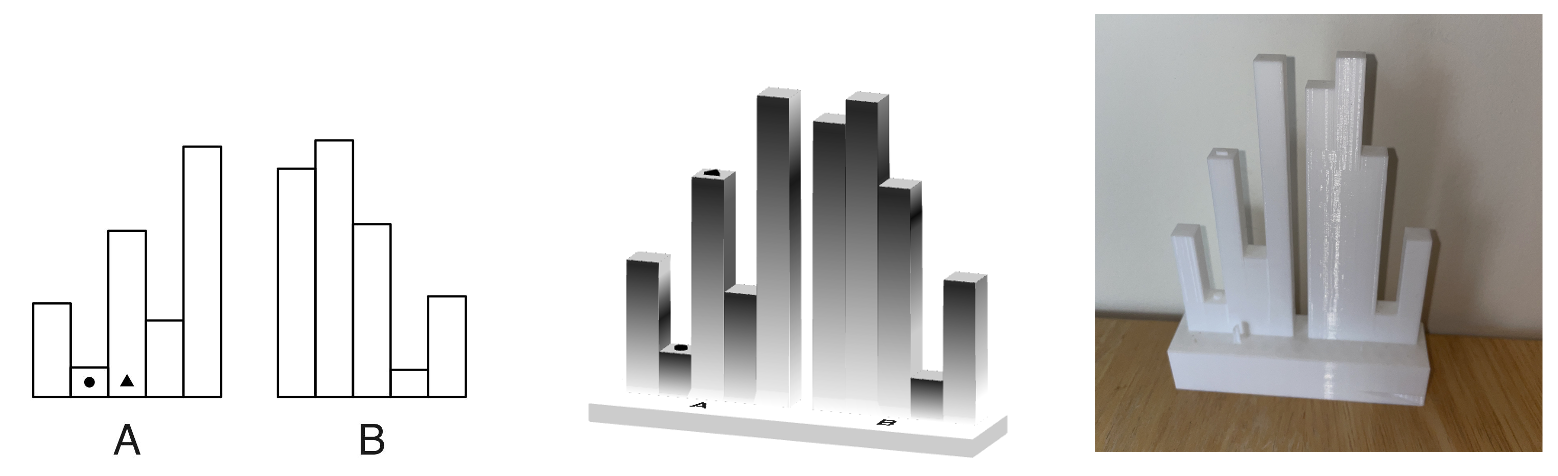
\includegraphics[width=\columnwidth]{chart_types}}
\caption{A 2D graph, 3D graph, and a prototype 3D printed graph showing the same set of data.}
\label{chartcomparison}
\end{center}
\end{figure}
The ggplot2 package was utilized to create the 2D bar charts.
The scale axis was removed, leaving only the bars and a bar grouping identifier. 
The values of comparison are marked by either a circle or a triangle at a height of 5 out of 100, which was estimated from Cleveland and McGill's paper using pixel ratio approximations.

For the 3D bar charts, the rayshader package was used. 
The graphs were created by using tiles with the fill color corresponding to height.
The fill color scale limits are identified by the same color on a scale from 0 to 100 in order for rayshader to map the fill to height.
A small space was added between the tiles since these sometimes caused triangular planes to appear when rendering to an RGL device
The scaling of the height from rayshader was determined by saving plots from a direct viewing angle and comparing aspect ratios of the height of one bar to the width of all bars as measured by pixel distances to the equivalent 2D data representation. 
However, small discrepancies exist for the scaling factor for different bar heights, so one of the "middle" bar heights of 26.1 to determine the final scale parameter. 
The values of comparison were identified by placing the circle and triangle on top of the corresponding bar.

For the 3D printed charts, the identifying marks were raised by a marginal amount so that they can be immediately identified after printing. 
Other non-data related elements were also raised for the same reason.
A negative-space engraving on the bottom of the 3D printed graph uniquely identifies each graph.
Graphs were printed with colored filament that correspond to a color coordinated ratio comparison.
The ratios were randomly assigned a unique color so that the color does not provide an indication as to what ratio is conveyed.

The digital 3D charts are initially angled to mimic the default 3D bar charts of Microsoft Excel, but the interactivity of Shiny will allow users to adjust the viewing angle. 
For a homogeneous appearance of data elements, a solid light grey appearance was used for the digital 3D representation, and the identifiers were marked black indicators for comparison.

\subsection{Study Design}

In the spirit of replicating Cleveland and McGill's study, members of our Statistics department and their spouses/partners were asked to participate in our study.
Participants are provided a single kit that has five of seven unique ratio comparisons where each ratio is applied to all three chart types. 
There are 21 kits in total so that each combination of ratios is accounted for.
Each graph is randomly assigned either an adjacent or separated comparison.

A Shiny application on a single computer is used to administer the graphs and questions to participants in a random order. 
Participants are provided a few sample graphs before receiving the graphs in their randomly assigned kit.
Prior to answering questions, participants are instructed to make quick judgements for each graph and not to estimate the ratios using physical objects, such as their fingers or pencils.
For the 3D printed graphs, the Shiny application directs participants to a colored graph in a bag and to verify the identifier on the bottom of the graph. 

Each graph has two accompanying questions asking which bar is smaller and what the ratio of the smaller bar is to the larger bar. 
Participants are presented radio buttons to identify the smaller bar and a slider to input a ratio judgement.

The responses will be measured by log error of the distance between the true ratio and the participant ratio judgement.
$$\text{Response}=\text{log}_2(|\text{judged percent}-\text{true percent}|+1/8)$$

At SDSS, the results will be presented, the implications of the charts will be assessed, and it will be reflected upon what this means for 3D charts.

\section{Future Research and Implications}

We hope to be able to extend our study into the curriculum of an introductory statistics course for Spring 2023.
The larger sample size will help to establish the perceptual difference of position along common scale judgements between 2D, 3D, and 3D printed bar charts. 
Should the results of the larger study show an improvement of 3D printed charts over 3D charts rendered in 2D, then we will have shown that the largely negative view of 3D graphs is slightly misguided. 
These results will extend into further 3D printed graphics research and possibly provide support for creating data graphics for the visually impaired.

At the final conclusion of the study, we will release a repository to encourage replication and the sharing of experimental results.

\bibliographystyle{sdss2020} % Please do not change the bibliography style
\bibliography{SDSS2023_AbstractReferences}

\end{document}
